\documentclass[letterpaper, 10 pt, conference]{ieeeconf}
  % use above line letter sized paper
%\documentclass[a4paper, 10pt, conference]{ieeeconf}
  % Use this line for a4 paper
%\IEEEoverridecommandlockouts
  % Needed if you want to use the \thanks command
\overrideIEEEmargins
  % Needed to meet printer requirements.
\usepackage[utf8]{inputenc}
\usepackage{fullpage}
\usepackage{graphicx}
\usepackage{amsfonts}
\usepackage{amssymb}
\usepackage{amsmath}
\usepackage{latexsym}
\usepackage{enumerate}
\usepackage{float}
\usepackage[urlcolor=blue,colorlinks=true]{hyperref}
\usepackage{multirow}
\usepackage{leftidx}
\usepackage[backend=bibtex,
style=numeric
%style=alphabetic
%style=reading
]{biblatex}
\addbibresource{Sources.bib}

\title{Conversion of RGBD Images to Textured Triangle Meshes with GPU}
\author{Dalton Banks, Collin Boots}
\date{Nov 18, 2013}
\begin{document}
   \maketitle


\section{Background} 
Previous work has demonstrated the diverse capabilities of RGBD cameras, from generating highly accurate 3D surface models to reliable 3D pose estimation. However, many algorithms attempt to store the generated environment as a RGB 3D point cloud, which is not easily adaptable to dynamic environments, requires very large quantities of memory to store large environments, and provides no intuition to higher perception processes about distinct objects beyond a volumetric approximation. Other approaches have been able to store and merge the surface data more efficiently, but still regard the environement as a unified whole rather than discrete objects. By extracting meaningful geometry from the RGB-D in the form of triangle meshes instead, a large number of advantages can be realized.

\begin{enumerate}
\item High storage efficiency
\item Natural low level object segmentation
\item Easy to manipulate, modify, and render in real time
\item Efficient and easy to process intuition of geometry that higher cognitive functions can use for object recognition and manipulation tasks.
\item Straightforward tradeoff between simplicity and accuracy with mesh resolution
\end{enumerate}

\section{Project Scope}
For this project, a segment of the pipeline will be implemented utilizing CUDA/OpenGL powered GPU acceleration (Figure \ref{fig:pipeline}).  Each segment of the pipeline has elements which may benefit from GPU acceleration. Blue segments are trivial functions that are easy to implement in CUDA/OpenGL. The red block represets the actual mesh generatation; this is the most complicated part of the pipeline and the main focus of the project. Green blocks represent stretch goals for the project, and are not strictly needed for the pipeline to function. A finished demo of the project would include side by side comparison of the raw kinect data and rendered mesh.

\begin{figure}[!ht]
    \centering
    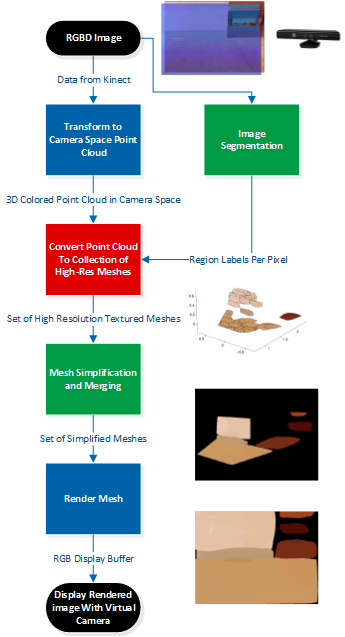
\includegraphics[scale=1.0]{pipelineflowchart.png}
    \caption{Pipeline Overview}
    \label{fig:pipeline}
\end{figure}

%\printbibliography
\end{document}